\documentclass{beamer}

\usepackage{cmap}				% To be able to copy-paste russian text from pdf
\usepackage[T2A]{fontenc}
\usepackage[utf8]{inputenc}
\usepackage[english]{babel}
\usepackage{textpos}
\usepackage{ragged2e}
\usepackage{amssymb}
\usepackage{ulem}
\usepackage{tikz}
\usepackage{pgfplots}
\usepackage{color}
\usepackage{cancel}
\usepackage{multirow}
\pgfplotsset{compat=1.17}
\usetikzlibrary{arrows,snakes,backgrounds,shapes}
\usepgfplotslibrary{groupplots,colorbrewer,dateplot,statistics}
\usepackage{animate}

\usepackage{amsfonts}
\usepackage{amsmath}
\usepackage{amssymb}
\usepackage{graphicx}
\usepackage{setspace}
\usepackage{cancel}

\usepackage{enumitem}
\setitemize{label=\usebeamerfont*{itemize item}%
  \usebeamercolor[fg]{itemize item}
  \usebeamertemplate{itemize item}}

% remove navigation bar
\setbeamertemplate{navigation symbols}{} 

\usepackage{eurosym}
\renewcommand{\EUR}[1]{\textup{\euro}#1}

\title{Options and the Binomial Model}
\author{Artem Bakulin}
\date{October 26, 2023}

\usetheme{Warsaw}
\usecolortheme{beaver}

\setbeamertemplate{page number in head/foot}[totalframenumber] 
\begin{document}



\begin{frame}
\titlepage
\end{frame}



\begin{frame}{Options}
\justifying
A \alert{call  [put] option} is a contract which grants the owner the right, but not the obligation, to buy [to sell] an underlying asset at a specified price on a specified date.

\justify
An example: a call option which allows to buy 1\,000 EUR for 1\,060 USD in 3 months. Today one would need to pay 20 USD for such an option.
\end{frame}



\begin{frame}{Options - 2}
\begin{itemize}
\justifying
\item A \alert{call} option gives the right to buy, a \alert{put} option gives the right to sell.
\item \alert{Strike} is the specified price at which holder of an option may buy the underlying asset.
\item \alert{Premium} is the amount which one needs to pay today to become holder of an option.
\item To \alert{write} an option is the same as selling an option.
\item \alert{Expiration date} is a date on which an option ceases to exist in case the holder did not exercise his right.
\item A \alert{European} option can only be exercised on the expiration date.
\item An \alert{American} option can be exercised on any day prior to the expiration date.
\end{itemize}
\end{frame}



\newcommand{\circlewithtext}[3]{
    \node[circle, fill, inner sep = 1.5pt] at (#1, #2) {};
    \node[anchor = north] at (#1, #2) {#3};
}

\begin{frame}{Foreign exchange options}
\justify
\centering
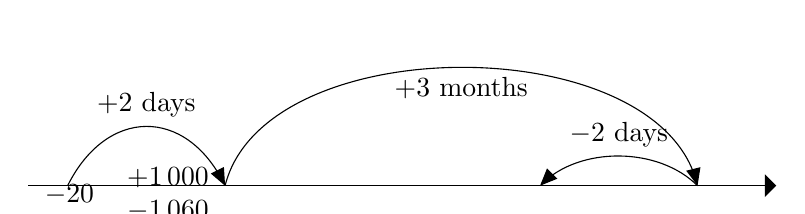
\begin{tikzpicture}
		\draw [->,>=triangle 90] (0, 0) -- (9.5, 0);
		
		\draw [->, >=triangle 45] (0.5, 0) .. controls (1.0, 1) and (2.0, 1) .. (2.5, 0) node[pos=0.5, anchor=south]{+2 days};
		
		\draw [->, >=triangle 45] (2.5, 0) .. controls (3, 2) and (8, 2) .. (8.5, 0) node[pos=0.5, anchor=north]{+3 months};
		
		\draw [->, >=triangle 45] (8.5, 0) .. controls (8, 0.5) and (7, 0.5) .. (6.5, 0) node[pos=0.5, anchor=south]{$-2$ days};
		
		\circlewithtext{0.5}{0}{Today};
		\circlewithtext{2.5}{0}{\begin{tabular}{c}Spot \\ $-20$ USD\end{tabular}};
		\circlewithtext{6.5}{0}{Expiration};
		\circlewithtext{8.5}{0}{\begin{tabular}{c}Settlement \\ $+1\,000$ EUR\\ $-1\,060$ USD\end{tabular}};
	\end{tikzpicture}
	
\justify
\begin{itemize}
\justifying
\item A buyer and a seller negotiate and sign a contract \alert{today}.
\item The buyer pays the premium on the \alert{spot date} (usually T+2).
\item The buyer has to inform the seller about exercising the option on the \alert{expiration date}.
\item If the option is exercised, the currency exchange happens on the \alert{settlement date}.
\end{itemize}

\justify
In this course we assume that the premium is paid today, and that settlement date is the same as expiation date.
\end{frame}



\begin{frame}{Vanilla options}
\justify
European options are often called \alert{plain vanilla} options because vanilla ice cream is the most common kind of ice cream.

\justify
Russian state television about Societe General's losses (2008):

\justify
"A source within the bank, under the condition of anonymity, informed Reuters that the trader in question has been recently buying and selling contracts for the delivery of plain vanilla ---\alert{ the kind used in cooking}. However, it's worth noting that vanilla production worldwide doesn't reach 7 billion dollars annually. Essentially, this is a form of trading in thin air, though it's entirely legal and widely practiced."

\justify
\url{https://www.newsru.com/russia/25Jan2008/vanilla.html}
\end{frame}



\begin{frame}{Example: call options}
\justifying
Owning a EURUSD call option to buy 100 EUR at strike 1.06.

\justifying
\centering
	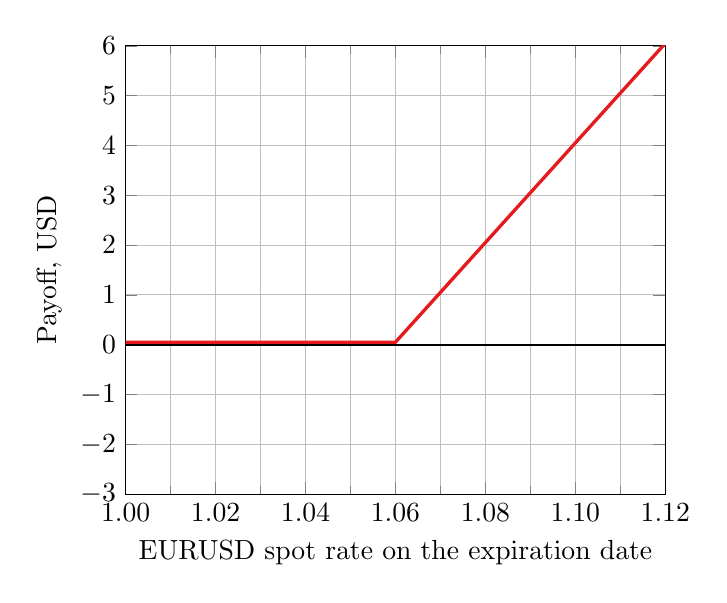
\begin{tikzpicture}
		\begin{axis}[
			domain=1:1.12,
			xmin=1, xmax=1.12,			
			xtick distance = 0.02,
			minor x tick num=1,
			ymin=-3, ymax=6,
			ytick distance = 1,
			grid = both,
			xlabel={EURUSD spot rate on the expiration date},
			ylabel={Payoff, USD},
 			x tick label style={
				/pgf/number format/.cd,
				fixed,
          			fixed zerofill,
				precision = 2
			}
     ]
		]
  \addplot[Set1-A, very thick] {100*(\x > 1.06)*(\x - 1.06) + 0.05};
  
  \draw[thick, color=black] (axis cs: 0, 0) -- (axis cs: 2, 0);
\end{axis}
\end{tikzpicture}
\end{frame}



\begin{frame}{Buying call options}
\justifying
Buying 100 EURUSD call options: strike 1.06, premium 2 USD.

\justifying
\centering
	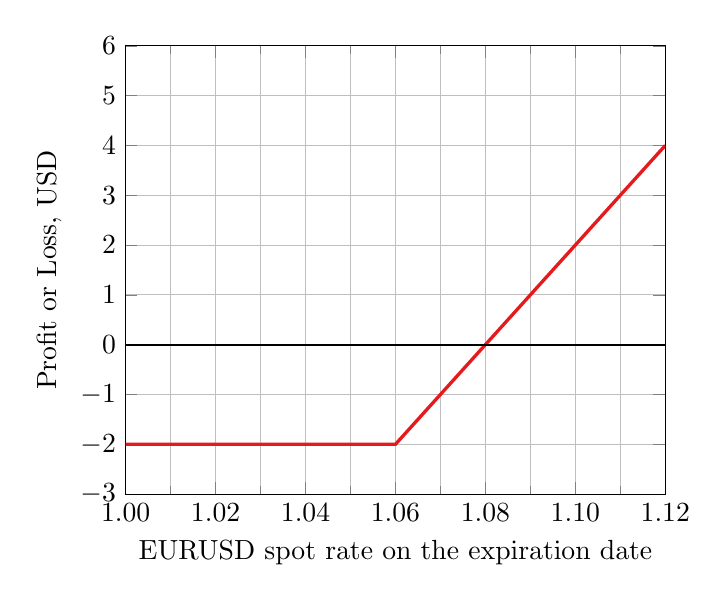
\begin{tikzpicture}
		\begin{axis}[
			domain=1:1.12,
			xmin=1, xmax=1.12,			
			xtick distance = 0.02,
			minor x tick num=1,
			ymin=-3, ymax=6,
			ytick distance = 1,
			grid = both,
			xlabel={EURUSD spot rate on the expiration date},
			ylabel={Profit or Loss, USD},
 			x tick label style={
				/pgf/number format/.cd,
				fixed,
          			fixed zerofill,
				precision = 2
			}
     ]
		]
  \addplot[Set1-A, very thick] {100*(\x > 1.06)*(\x - 1.06) - 2};
  
  \draw[thick, color=black] (axis cs: 0, 0) -- (axis cs: 2, 0);
\end{axis}
\end{tikzpicture}
\end{frame}



\begin{frame}{Buying put options}
\justifying
Buying 100 EURUSD put options: strike 1.06, premium 2 USD.

\justifying
\centering
	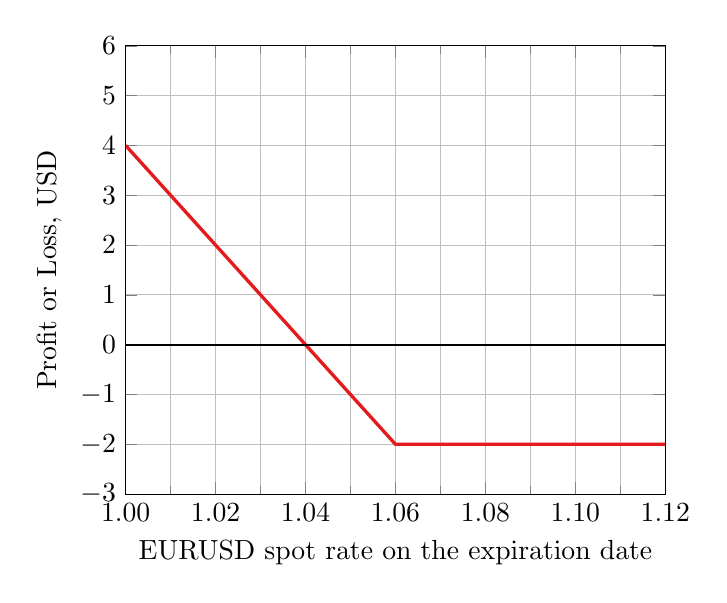
\begin{tikzpicture}
		\begin{axis}[
			domain=1:1.12,
			xmin=1, xmax=1.12,			
			xtick distance = 0.02,
			minor x tick num=1,
			ymin=-3, ymax=6,
			ytick distance = 1,
			grid = both,
			xlabel={EURUSD spot rate on the expiration date},
			ylabel={Profit or Loss, USD},
 			x tick label style={
				/pgf/number format/.cd,
				fixed,
          			fixed zerofill,
				precision = 2
			}
     ]
		]
  \addplot[Set1-A, very thick] {100*(\x < 1.06)*(1.06 - \x ) - 2};
  
  \draw[thick, color=black] (axis cs: 0, 0) -- (axis cs: 2, 0);
\end{axis}
\end{tikzpicture}
\end{frame}



\begin{frame}{Selling call options}
\justifying
Selling 100 EURUSD call options: strike 1.06, premium 2 USD.

\justifying
\centering
	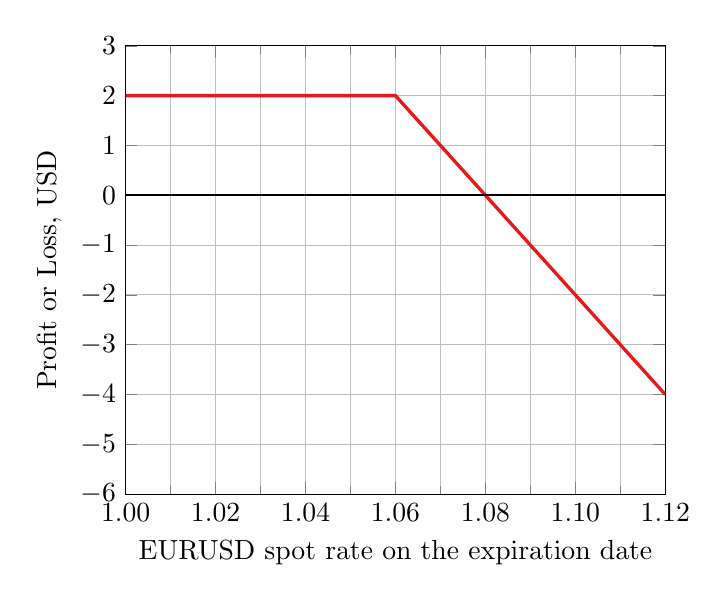
\begin{tikzpicture}
		\begin{axis}[
			domain=1:1.12,
			xmin=1, xmax=1.12,			
			xtick distance = 0.02,
			minor x tick num=1,
			ymin=-6, ymax=3,
			ytick distance = 1,
			grid = both,
			xlabel={EURUSD spot rate on the expiration date},
			ylabel={Profit or Loss, USD},
 			x tick label style={
				/pgf/number format/.cd,
				fixed,
          			fixed zerofill,
				precision = 2
			}
     ]
		]
  \addplot[Set1-A, very thick] {-100*(\x > 1.06)*(\x - 1.06) + 2};
  
  \draw[thick, color=black] (axis cs: 0, 0) -- (axis cs: 2, 0);
\end{axis}
\end{tikzpicture}
\end{frame}



\begin{frame}{Selling put options}
\justifying
Selling 100 EURUSD put options: strike 1.06, premium 2 USD.

\justifying
\centering
	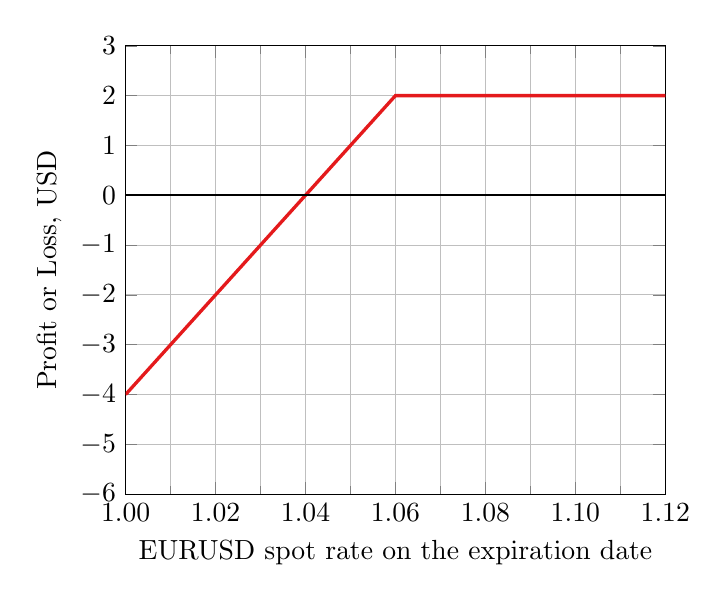
\begin{tikzpicture}
		\begin{axis}[
			domain=1:1.12,
			xmin=1, xmax=1.12,			
			xtick distance = 0.02,
			minor x tick num=1,
			ymin=-6, ymax=3,
			ytick distance = 1,
			grid = both,
			xlabel={EURUSD spot rate on the expiration date},
			ylabel={Profit or Loss, USD},
 			x tick label style={
				/pgf/number format/.cd,
				fixed,
          			fixed zerofill,
				precision = 2
			}
     ]
		]
  \addplot[Set1-A, very thick] {-100*(\x < 1.06)*(1.06 - \x ) + 2};
  
  \draw[thick, color=black] (axis cs: 0, 0) -- (axis cs: 2, 0);
\end{axis}
\end{tikzpicture}
\end{frame}



\begin{frame}{Hedging with call options}
\justify
In 3 months we will need 1\,000 EUR. Forward rate for the 3 months maturity is 1.06. We could buy a forward, but we wary about EUR possibly depreciating to 1.00. It will be a disappointment to buy EURUSD at 1.06 when the market will be trading at 1.00.

\justify
Solution: we can buy 1\,000 call options at the strike of 1.06 for the premium of 20 USD. In the event of EURUSD appreciation we can exercise our option and buy at 1.06. If the EUR suddenly weakens, we let the option expire and buy EURUSD at the prevailing market rate of 1.00.

\justify
Pros: we do not suffer from EURUSD depreciation. Cons: we have to pay a premium upfront. This option is our insurance against EURUSD rising higher than 1.06.
\end{frame}




\begin{frame}{Hedging with put options}
\justify
In 3 months we will receive 1\,000 EUR. Forward rate for the 3 months maturity is 1.06. If we sell a forward we secure the exchange rate, but expose ourselves to the EUR appreciating to 1.12 or higher. We will have to sell EURUSD at 1.06 when everyone around will be happily trading at 1.12.

\justify
Solution: we can buy 1\,000 put options at the strike of 1.06 for the premium of 20 USD. In case the EUR depreciates to 1.00 we exercise the option and sell at 1.06. In case EURUSD jumps to 1.12 we let the option expire and sell at the prevailing rate of 1.12

\justify
Pros: we will not be disappointed in the event of the EUR appreciation. Cons: we have to pay a premium upfront. The option protects us from the EURUSD dropping below 1.06.
\end{frame}



\begin{frame}{Speculating with call options}
\justify
A crystal ball shows that in 3 months EURUSD will significantly \alert{appreciate} from the current level of 1.06. We are willing to monetize this forecast. However \sout{the wife} shareholders in our hedge fund allocated the budget of just 20 USD.

\justify
Solution: we can buy 1\,000 EURUSD \alert{call} options at the strike of 1.06 for the premium of 20 USD. In case EURUSD appreciates to 1.16 we can make $(1.16 - 1.06) \cdot 1\,000 - 20 = 80$ USD. If this does not happen we just lose our bet of 20 USD which is within our risk budget.

\justify
An option acts as a leverage. It magnifies both the profit in positive scenarios (as if we had 1\,000 EUR to bet) and the loss in negative scenarios (we can lose the whole premium). Good news is that the loss is floored at the premium, but the gain is potentially unlimited.
\end{frame}



\begin{frame}{Speculating with put options}
\justify
A crystal ball suggests that in 3 months EURUSD will \alert{depreciate} relative to the current forward rate of 1.06. Our shareholders allocated a budget of 20 USD to let us monetize this forecast.

\justify
Solution: we can buy 1\,000 EURUSD \alert{put} options at the strike of 1.06 for the premium of 20 USD. If we are right and EURUSD depreciates to 0.96 we can make $(1.06 - 0.96)\cdot1\,000 - 20 = 80$ USD. If this does not happen we simply lose the premium.

\justify
A put option allows betting on depreciation of the underlying asset (of the EUR).
\end{frame}



\begin{frame}{Moneyness}
\justify
There are three standard terms for the \alert{moneyness} of call options:

\begin{itemize}
\justifying
\item In the money, ITM --- current spot price of the underlying asset is higher than the strike (it would be profitable to exercise the option immediately).
\item At the money, ATM --- current spot price is equal to the strike.
\item Out of the money, OTM --- current spot price of the underlying asset is lower than the strike (it would be unprofitable to exercise the option immediately).
\end{itemize}

\justify
There are symmetrical terms for put option.
\end{frame}



\begin{frame}{Combinations: a collar}
\justifying
A \alert{collar} consists of a sold put at a lower strike and a bought call at a higher strike.

\justifying
\centering
	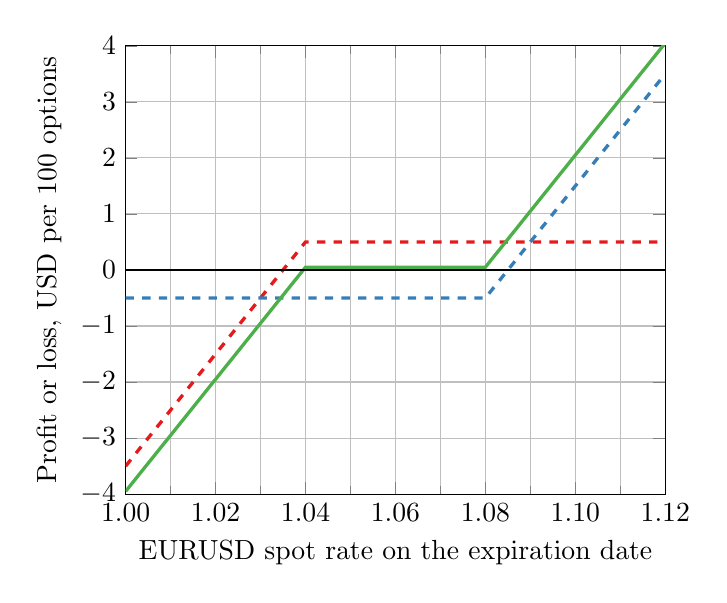
\begin{tikzpicture}
		\begin{axis}[
			domain=1:1.12,
			xmin=1, xmax=1.12,			
			xtick distance = 0.02,
			minor x tick num=1,
			ymin=-4, ymax=4,
			ytick distance = 1,
			grid = both,
			xlabel={EURUSD spot rate on the expiration date},
			ylabel={Profit or loss, USD per 100 options},
 			x tick label style={
				/pgf/number format/.cd,
				fixed,
          			fixed zerofill,
				precision = 2
			}
		]
	
  \addplot[Set1-A, very thick, dashed] {-100*(\x < 1.04)*(1.04 - \x) + 0.5};
  \addplot[Set1-B, very thick, dashed] {100*(\x > 1.08)*(\x - 1.08) - 0.5};
  \addplot[Set1-C, very thick] {-100*(\x < 1.04)*(1.04 - \x) + 0.5 + 100*(\x > 1.08)*(\x - 1.08) - 0.5 + 0.05};	

  \draw[thick, color=black] (axis cs: 0, 0) -- (axis cs: 1.12, 0);
\end{axis}
\end{tikzpicture}
\end{frame}



\begin{frame}{Combinations: a call spread}
\justifying
A \alert{call spread} consists of a bought call at a lower strike and a sold call at a higher strike.

\justifying
\centering
	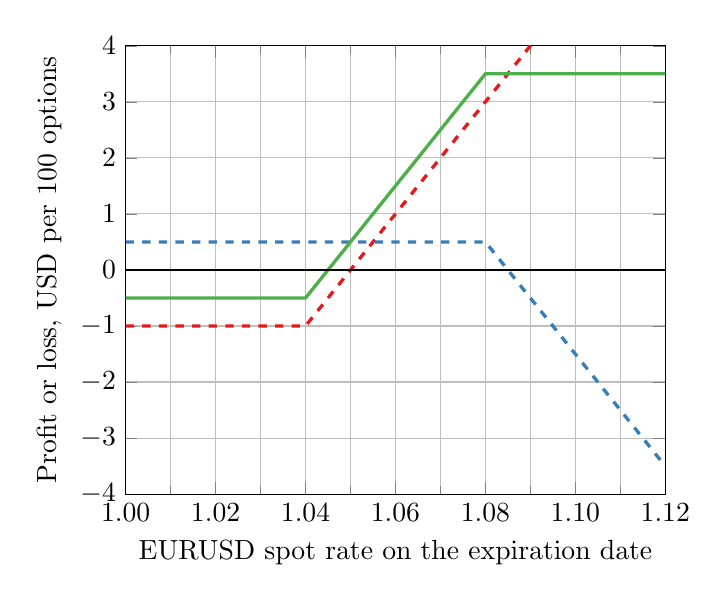
\begin{tikzpicture}
		\begin{axis}[
			domain=1:1.12,
			xmin=1, xmax=1.12,			
			xtick distance = 0.02,
			minor x tick num=1,
			ymin=-4, ymax=4,
			ytick distance = 1,
			grid = both,
			xlabel={EURUSD spot rate on the expiration date},
			ylabel={Profit or loss, USD  per 100 options},
 			x tick label style={
				/pgf/number format/.cd,
				fixed,
          			fixed zerofill,
				precision = 2
			}
		]
		
	  \addplot[Set1-A, very thick, dashed] {100*(\x > 1.04)*(\x - 1.04) - 1};
  \addplot[Set1-B, very thick, dashed] {-100*(\x > 1.08)*(\x - 1.08) + 0.5};
  \addplot[Set1-C, very thick] {100*(\x > 1.04)*(\x - 1.04) - 1 - 100*(\x > 1.08)*(\x - 1.08) + 0.5};
  
  \draw[thick, color=black] (axis cs: 1, 0) -- (axis cs: 2, 0);
\end{axis}
\end{tikzpicture}
\end{frame}



\begin{frame}{Combinations: a straddle}
\justifying
A \alert{straddle} is a bought call and a bought put at equal strikes.

\justifying
\centering
	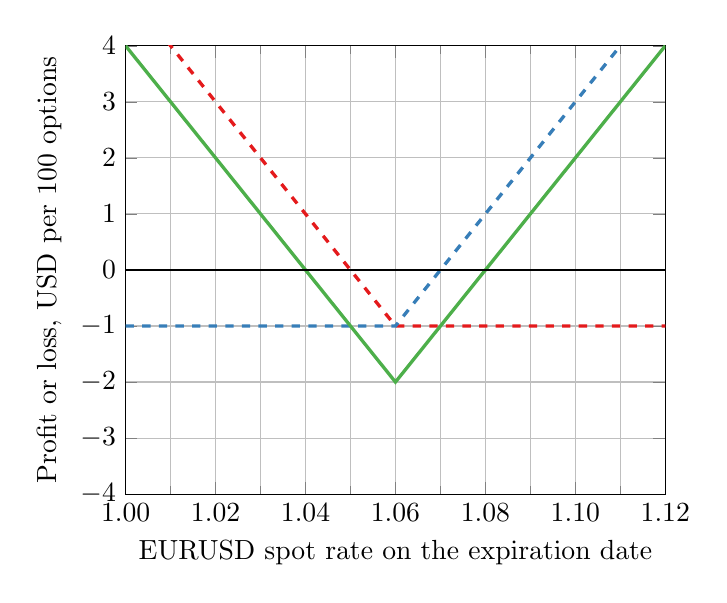
\begin{tikzpicture}
		\begin{axis}[
			domain=1:1.12,
			xmin=1, xmax=1.12,			
			xtick distance = 0.02,
			minor x tick num=1,
			ymin=-4, ymax=4,
			ytick distance = 1,
			grid = both,
			xlabel={EURUSD spot rate on the expiration date},
			ylabel={Profit or loss, USD  per 100 options},
 			x tick label style={
				/pgf/number format/.cd,
				fixed,
          			fixed zerofill,
				precision = 2
			}
		]
		
	  \addplot[Set1-A, very thick, dashed] {100*(\x < 1.06)*(1.06 - \x) - 1};
  \addplot[Set1-B, very thick, dashed] {100*(\x > 1.06)*(\x - 1.06) - 1};
  \addplot[Set1-C, very thick] {100*(\x < 1.06)*(1.06- \x) - 1 + 100*(\x > 1.06)*(\x - 1.06) - 1};
  
  \draw[thick, color=black] (axis cs: 1, 0) -- (axis cs: 2, 0);
\end{axis}
\end{tikzpicture}
\end{frame}



\begin{frame}{Combinations: a call and a put}
\justifying
Buying a call and selling a put at the same strike.

\justifying
\centering
	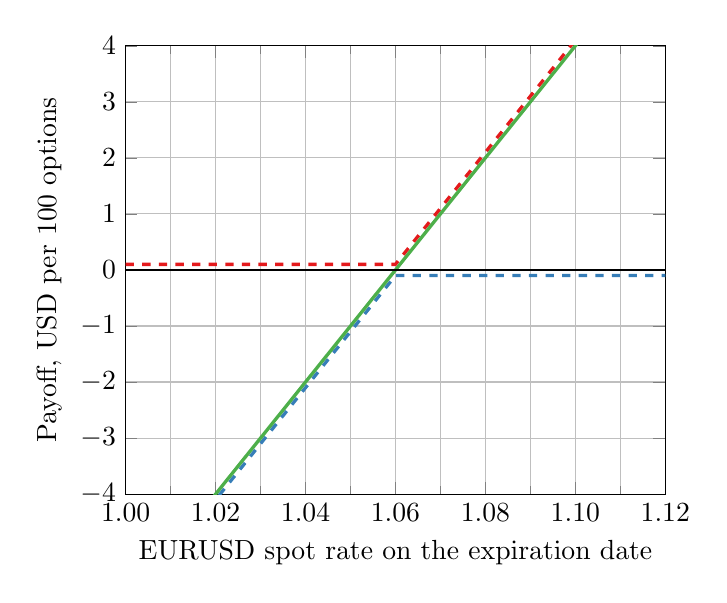
\begin{tikzpicture}
		\begin{axis}[
			domain=1:1.12,
			xmin=1, xmax=1.12,			
			xtick distance = 0.02,
			minor x tick num=1,
			ymin=-4, ymax=4,
			ytick distance = 1,
			grid = both,
			xlabel={EURUSD spot rate on the expiration date},
			ylabel={Payoff, USD  per 100 options},
 			x tick label style={
				/pgf/number format/.cd,
				fixed,
          			fixed zerofill,
				precision = 2
			}
		]
		
	\addplot[Set1-A, very thick, dashed] {100*(\x > 1.06)*(\x - 1.06) + 0.1};
  	\addplot[Set1-B, very thick, dashed] {-100*(\x < 1.06)*(1.06-\x) - 0.1};
  	\addplot[Set1-C, very thick] {100*(\x > 1.06)*(\x - 1.06) - 100*(\x < 1.06)*(1.06-\x) };
 
   \draw[thick, color=black] (axis cs: 1, 0) -- (axis cs: 2, 0);
\end{axis}
\end{tikzpicture}
\end{frame}



\begin{frame}{Combinations: underlying asset and debt}
\justifying
100 EUR on bank account and debt of 106 USD

\justifying
\centering
	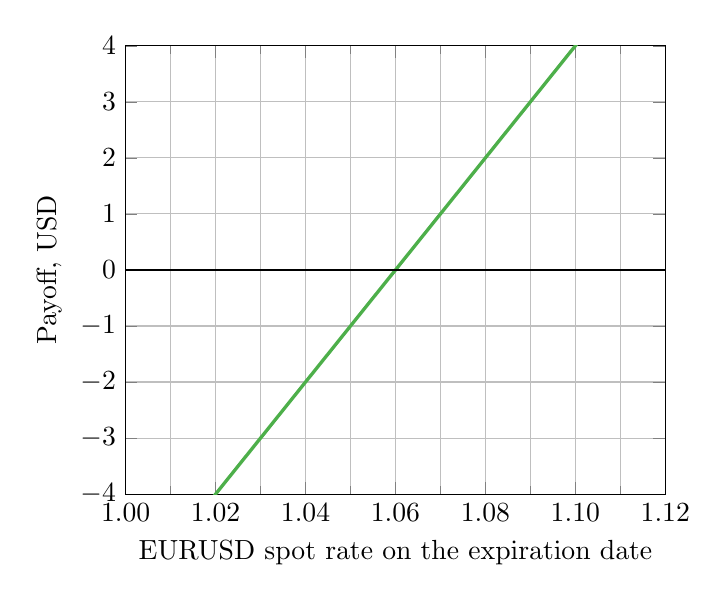
\begin{tikzpicture}
		\begin{axis}[
			domain=1:1.12,
			xmin=1, xmax=1.12,			
			xtick distance = 0.02,
			minor x tick num=1,
			ymin=-4, ymax=4,
			ytick distance = 1,
			grid = both,
			xlabel={EURUSD spot rate on the expiration date},
			ylabel={Payoff, USD},
 			x tick label style={
				/pgf/number format/.cd,
				fixed,
          			fixed zerofill,
				precision = 2
			}
		]
		
  	\addplot[Set1-C, very thick] {100*(\x - 1.06)};
 
   \draw[thick, color=black] (axis cs: 1, 0) -- (axis cs: 2, 0);
\end{axis}
\end{tikzpicture}
\end{frame}



\begin{frame}{Call-put parity}
\justify
The following two portfolios yield identical payoffs on the expiration date $T$:
\begin{itemize}
\justifying
\item Bought call at strike $K$ and sold put at strike $K$.
\item Underlying asset at price $S(T)$ and debt of $K$ units of cash.
\end{itemize}

\justify
Consequently, on any day $t$ prior to the expiration date ($t<T$) these portfolios should be priced equally, taking the discount rate $r$ into account (*):
\begin{align*}
C_K(t) - P_K(t) = S(t) - Ke^{-r(T-t)}
\end{align*}

\justify
This equation is called the \alert{call-put parity}. We can derive fair value of a put from fair value of a call, and vice versa.

\justify
(*) In case the underlying asset pays continuously compounded dividend yield $q$ (e.g. interest rate in EUR):
\begin{align*}
C_K(t) - P_K(t) = S(t)e^{-q(T-t)} - Ke^{-r(T-t)}
\end{align*}
\end{frame}



\begin{frame}{Digital options}
\justify
A European \alert{digital call [put]} option is a contract that entitles the buyer receive a fixed payment in case the price of the underlying asset on the expiration date is higher [lower] than the specified strike.

\justify
An example: a European digital call option at strike of 1.06, expiration in 3 months, and notional amount of 100 USD. 

\justify
The buyer will receive 100 USD from the seller in 3 months if the prevailing EURUSD spot rate will be higher than 1.06.
\end{frame}



\begin{frame}{Buying a digital call option}
\justifying
Buying a digital call: strike is 1.06, notional amount is 1 USD.

\justifying
\centering
	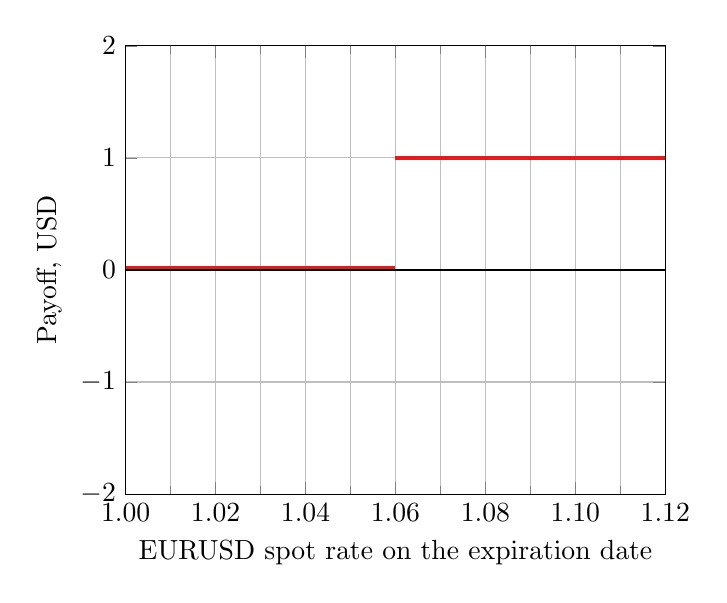
\begin{tikzpicture}
		\begin{axis}[
			domain=1:1.12,
			xmin=1, xmax=1.12,			
			xtick distance = 0.02,
			minor x tick num=1,
			ymin=-2, ymax=2,
			ytick distance = 1,
			grid = both,
			xlabel={EURUSD spot rate on the expiration date},
			ylabel={Payoff, USD},
 			x tick label style={
				/pgf/number format/.cd,
				fixed,
          			fixed zerofill,
				precision = 2
			}
		]
		
	\addplot[Set1-A, very thick, domain=1.06:1.12] {1};
	\addplot[Set1-A, very thick, domain=1:1.06] {0.02};
 
   \draw[thick, color=black] (axis cs: 1, 0) -- (axis cs: 2, 0);
\end{axis}
\end{tikzpicture}
\end{frame}



\begin{frame}{Buying a digital put option}
\justifying
Buying a digital put: strike is 1.06, notional amount is 1 USD.

\justifying
\centering
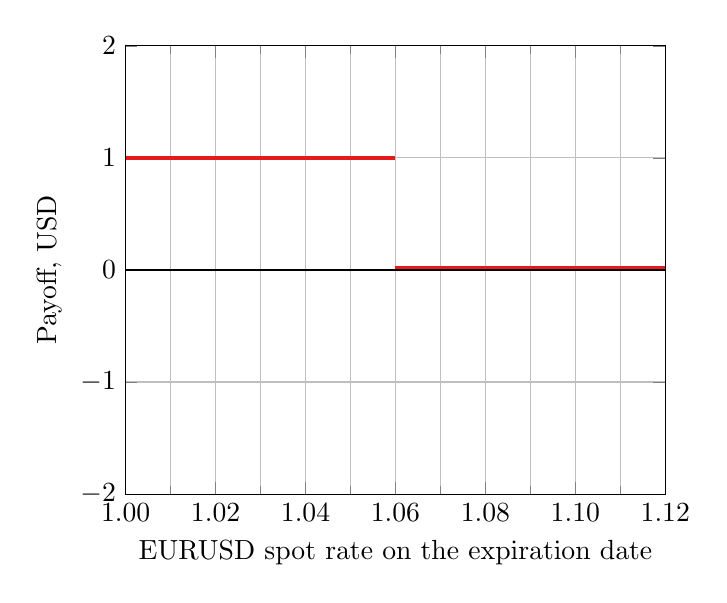
\begin{tikzpicture}
		\begin{axis}[
			domain=1:1.12,
			xmin=1, xmax=1.12,			
			xtick distance = 0.02,
			minor x tick num=1,
			ymin=-2, ymax=2,
			ytick distance = 1,
			grid = both,
			xlabel={EURUSD spot rate on the expiration date},
			ylabel={Payoff, USD},
 			x tick label style={
				/pgf/number format/.cd,
				fixed,
          			fixed zerofill,
				precision = 2
			}
		]
		
	\addplot[Set1-A, very thick, domain=1.00:1.06] {1};
	\addplot[Set1-A, very thick, domain=1.06:1.12] {0.02};
 
   \draw[thick, color=black] (axis cs: 1, 0) -- (axis cs: 2, 0);
\end{axis}
\end{tikzpicture}
\end{frame}



\begin{frame}{Speculating with digital options}
\justify
A digital option is a convenient tool for making speculative bets.

\justify
A crystal ball tells you that the exchange rate will be higher [lower] than a certain level. You are unsure whether it will be just a bit higher [lower] or much much higher [lower]. You are buying a digital call [put] to make a bet.

\justify
Pros: simple payoff chart, one can interpret the premium as probability of an event. Cons: it becomes difficult to hedge digital options in case the spot rate ends up close to the strike by the expiration date. Market-makers have to charge wider bid/ask spread to compensate for more expensive hedging.

\justify
Is there a link between price of a digital option and price of European vanilla options?
\end{frame}



\begin{frame}{A digital option and a call spread}
\justifying
\only<1>{Call spread: buy 100 calls-1.055, sell 100 calls-1.065}
\only<2>{Call spread: buy 200 calls-1.0575, sell 200 calls-1.0625}
\only<3>{Call spread: buy 1000 calls-1.0595, sell 1000 calls-1.0605}

\centering
	\begin{tikzpicture}
		\begin{axis}[
			domain=1.04:1.08,
			xmin=1.04, xmax=1.08,			
			xtick distance = 0.01,
			ymin=-1.5, ymax=1.5,
			ytick distance = 0.5,
			grid = both,
			xlabel={EURUSD spot rate on the expiration date},
			ylabel={Payoff, USD},
 			x tick label style={
				/pgf/number format/.cd,
				fixed,
          			fixed zerofill,
				precision = 2
			}
		]

\only<1>{
	\addplot[Set1-A, very thick, dashed] {100*(\x > 1.055)*(\x - 1.055) - 0.03};
  	\addplot[Set1-B, very thick, dashed] {-100*(\x > 1.065)*(\x - 1.065) + 0.06};
  	\addplot[Set1-C, very thick] {100*(\x > 1.055)*(\x - 1.055) - 100*(\x > 1.065)*(\x - 1.065) + 0.03};
}
\only<2>{
	\addplot[Set1-A, very thick, dashed, samples=100] {200*(\x > 1.0575)*(\x - 1.0575) - 0.03};
  	\addplot[Set1-B, very thick, dashed, samples=100] {-200*(\x > 1.0625)*(\x - 1.0625) + 0.06};
  	\addplot[Set1-C, very thick, samples=100] {200*(\x > 1.0575)*(\x - 1.0575) - 200*(\x > 1.0625)*(\x - 1.0625) + 0.03};
}
\only<3>{
	\addplot[Set1-A, very thick, dashed, samples=100] {1000*(\x > 1.0595)*(\x - 1.0595) - 0.03};
  	\addplot[Set1-B, very thick, dashed, samples=100] {-1000*(\x > 1.0605)*(\x - 1.0605) + 0.06};
  	\addplot[Set1-C, very thick, samples=100] {1000*(\x > 1.0595)*(\x - 1.0595) - 1000*(\x > 1.0605)*(\x - 1.0605) + 0.03};
}
 
   \draw[thick, color=black] (axis cs: 1, 0) -- (axis cs: 1.1, 0);
\end{axis}
\end{tikzpicture}
\end{frame}



\begin{frame}{Replicating a digital option}
\justify
We can approximately replicate a digital call option at strike $K$ with a vanilla call spread at strikes $K-\varepsilon$ and $K+\varepsilon$:
\begin{align*}
D(K) \approx nC\left(K - \dfrac{1}{2n}\right) - nC\left(K + \dfrac{1}{2n}\right)
\end{align*}
Here $C(K)$ is price of a European vanilla call at strike $K$, $D(K)$ is price of a digital call, $n$ is the number of vanilla calls in the call spread.

\justify
Fun fact: price of a digital call is the first derivative of the price of a vanilla call w.r.t. the strike.
\begin{align*}
D(K) = \lim\limits_{\varepsilon\to 0}\dfrac{C(K-\varepsilon) - C(K+\varepsilon)}{2\varepsilon} = -\dfrac{\partial C}{\partial K}
\end{align*}
\end{frame}



\begin{frame}{Call-put parity for digital options}
\justify
Consider a portfolio of a digital call and a digital put at the same strike:

\justify
\begin{itemize}
\justifying
\item The call pays 1 unit of a currency in case the price of the underlying asset is $\ge K$ (*).
\item The put pays 1 unit of a currency in case the price of the underlying asset is $< K$.
\end{itemize}

\justify
A portfolio of a digital put and a digital call always pays 1 unit of a currency. It is similar to a deposit at the risk-free rate $r$:
\begin{align*}
C_{digital}(K) + P_{digital}(K) = e^{-rT}
\end{align*}

\justify
(*) Suppose that the call pays 1 unit in case the spot rate hits the strike precisely.
\end{frame}



\begin{frame}{Barrier options}
\justify
A payoff on a \alert{barrier options} depends on whether the price of the underlying asset will take some specified values.

\justify
- \alert{Knock-in (KI)} barrier: an option begins to exist in case the spot price reaches the certain level.

- \alert{Knock-out (KO)} barrier: an option ceases to exist in case the spot price reaches the certain level.

\justify
- European barrier is only observed on the expiration date.

- American barrier is observed during the lifetime of the option.

- Window barrier is observed during a specified period.

\justify
Usually investors add barriers to their options to make the options cheaper.
\end{frame}


\begin{frame}{European knock-out (EKO)}
\justify
A call at strike 1.06 with a European knock-out barrier at 1.10.
\centering
	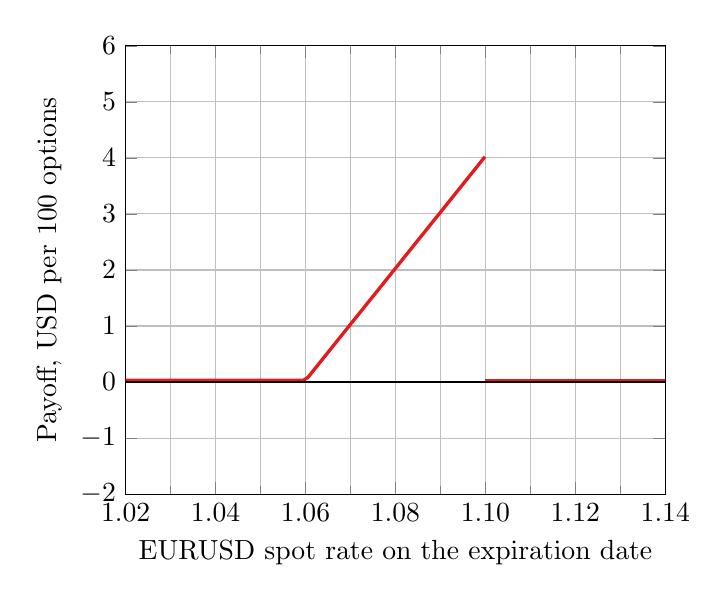
\begin{tikzpicture}
		\begin{axis}[
			domain=1.00:1.14,
			xmin=1.02, xmax=1.14,			
			xtick distance = 0.02,
			minor x tick num=1,
			ymin=-2, ymax=6,
			ytick distance = 1,
			grid = both,
			xlabel={EURUSD spot rate on the expiration date},
			ylabel={Payoff, USD per 100 options},
 			x tick label style={
				/pgf/number format/.cd,
				fixed,
          			fixed zerofill,
				precision = 2
			}
		]
  \addplot[Set1-A, very thick,domain=1:1.0999, samples=100] {100*(\x > 1.06)*(\x - 1.06) + 0.03};
  \addplot[Set1-A, very thick,domain=1.10:1.14] {0.03};
  
  \draw[thick, color=black] (axis cs: 1, 0) -- (axis cs: 1.2, 0);
\end{axis}
\end{tikzpicture}
\end{frame}



\begin{frame}{Replicating European options}
\justify
Payoff of a European-style derivative depends only on the price of the underlying asset on the expiration date. We can replicate any derivative of this kind with a combination of vanilla options and/or digital options.

\justify
1. Add a vanilla option at each point where the payoff chart bends.

\justify
2. Add a digital option at each point of discontinuity.

\justify
How do we replicate a European knock-out option at the strike at 1.06 with the barrier at 1.10?
\end{frame}



\begin{frame}{Replicating a European barrier}
\justify
Buy 100 vanilla calls-1.06
\only<2->{, sell 100 vanilla calls-1.10}
\only<3->{, sell 4 digital calls-1.10}
\justify
\centering
	\begin{tikzpicture}
		\begin{axis}[
			domain=1.00:1.14,
			xmin=1.02, xmax=1.14,			
			xtick distance = 0.02,
			minor x tick num=1,
			ymin=-5, ymax=5,
			ytick distance = 1,
			grid = both,
			xlabel={EURUSD spot rate on the expiration date},
			ylabel={Payoff, USD},
 			x tick label style={
				/pgf/number format/.cd,
				fixed,
          			fixed zerofill,
				precision = 2
			}
		]
  \addplot[Set1-A, very thick, dashed, samples=100] {100*(\x > 1.06)*(\x - 1.06) + 0.06};
\only<2->{
  \addplot[Set1-B, very thick, dashed] {-100*(\x > 1.10)*(\x - 1.10) - 0.03};
}
\only<2>{
  \addplot[Set1-C, very thick, samples=200] {-100*(\x > 1.10)*(\x - 1.10) - 0.03 + 100*(\x > 1.06)*(\x - 1.06) + 0.06};
}
\only<3->{
	\addplot[Set1-E, very thick, dashed, domain=1:1.10] {-0.06};
	\addplot[Set1-E, very thick, dashed, domain=1.10:1.14] {-4};
}
\only<3>{
	\addplot[Set1-C, very thick, domain=1:1.10, samples=200] {-100*(\x > 1.10)*(\x - 1.10) - 0.03 + 100*(\x > 1.06)*(\x - 1.06) + 0.06};
	\addplot[Set1-C, very thick, domain=1.10:1.14] {0.03};
}

  \draw[thick, color=black] (axis cs: 1, 0) -- (axis cs: 1.14, 0);
\end{axis}
\end{tikzpicture}
\end{frame}



\begin{frame}{Who is selling options?}
\justify
Options are convenient both for hedging and for speculation. Potential losses are floored, because a buyer cannot lose more than the premium. Potential gain of a call option is unlimited.

\justify
Who is selling options then? Who is ready to receive limited gain in exchange for unlimited losses?
\end{frame}



\begin{frame}{Who is selling options?}
\justify
In the past several option strategies resulted in positive average return in the long run.

\justify
\begin{itemize}
\justifying
\item Covered call: buy a stock market index, sell a call option at a high strike.
\item Short straddle: sell a straddle and delta-hedge it dynamically (later in this course).
\item Short OTM put: sell a put on a stock market index at a low strike (sell insurance against the market crash).
\end{itemize}

\justify
All three strategies are "selling the volatility". They bet that the market will not be fluctuating as much as option buyers anticipate. Options are similar to insurance. They are priced high enough so that sellers of the insurance may make money in the long run.
\end{frame}



\begin{frame}{Selling out-of-the money put}
\justify
S\&P\,500 index is currently at \$4\,120 (October 27, 2023). A put option at strike \$2\,700 which expires on December 15 is worth \$2 on Chicago Mercantile Exchange.

\justify
If you sell 1\,000 put options you collect the premium \$2\,000 with virtually no risk. Last time S\&P\,500 dropped by 35\% in 7 weeks in 1929 during the Great Depression.

\justify
Caveat: if the Great Depression comes back and the index drops to \$2\,600 you lose \$1\,000\,000.

\justify
Will you be brave enough to sell this insurance policy?

\justify
Could we do something less frightening?
\end{frame}



\begin{frame}{PUT Index}
\justify
The Chicago Board of Option Exchange  (CBOE) S\&P\,500 PutWrite Index ("PUT") tracks the following investment strategy.

\justify
1. Sell (write) a 1 month at-the-money put option on S\&P\,500 index. E.g. sell at strike $K=\$4\,120$ in case current level is \$4\,120.

\justify
2. Put aside $K$ dollars in risk-free one-month Treasury bills. Thus you will have cash at hand in case the index drops and the buyer exercises the option.

\justify
3. In good case you just collect the premium. In bad case you lose some money ($K-S$ where $S$ is index price), but you can never go below zero.

\justify
4. Repeat every month.
\end{frame}



\begin{frame}{PUT Index - 2}
\centering
\begin{tikzpicture}
\begin{axis}[
 	width=\textwidth,
	height=\textheight - 1cm,
	date coordinates in=x,
	date ZERO=1987-01-01,
  	xtick={1990-01-01, 2000-01-01, 2010-01-01, 2020-01-01},
  	minor xtick={1995-01-01, 2005-01-01, 2015-01-01, 2025-01-01},
  	xticklabel={\year},
  	xmin=1987-01-01,
  	xmax=2025-01-01,
	 ymode = log,
 	grid=both,
   	log ticks with fixed point,
  	ylabel={\small{Growth of \$1 investment}},
  	xlabel near ticks,
  	ylabel near ticks,
	legend entries = {
		S\&P\,500 Total Return,
		CBOE PUT Index,
		Risk-free T-bill
	},
	legend pos=north west,
	legend style={font=\scriptsize},
	legend cell align={left}
]

\addplot[color = Set1-A, mark = none, very thick]
	table[
		x=month,
		y=sp500_growth,
		col sep=comma
	]
	{cboe_puty.csv};

\addplot[color = Set1-B, mark = none, very thick]
	table[
		x=month,
		y=put_growth,
		col sep=comma
	]
	{cboe_puty.csv};

\addplot[color = Set1-C, mark = none, very thick, dashed]
	table[
		x=month,
		y=rf_growth,
		col sep=comma
	]
	{cboe_puty.csv};

   \draw[thick, color=black] (axis cs: 1985-01-01, 1) -- (axis cs: 2025-01-01, 1);
\end{axis}
\end{tikzpicture}
\small Data: CBOE, Robert Shiller, Kenneth French.
\end{frame}



\begin{frame}{PUT Index - 3}
\centering
\begin{tabular}{l|r|r|r}
& PUT & S\&P\,500 & T-bill \\ \hline
Geom. Mean & 9.3\% & 10.3\% & 2.9\% \\
Excess Return & 6.3\% & 7.2\% & 0.0\% \\
Std. Dev & 11.1\% & 16.2\% & 0.0\% \\
Share Ratio & 0.56 & 0.45 & 0.0 \\
Monthly Beta & 0.48 & 1.00 & 0.00
\end{tabular}

\small Sample period: 1987--2022. All figures except Beta are annualized.

\justify
PUT has better return to risk ratio (the Sharpe ratio). Insuring others from a stock market crash seems to be a better strategy than investing in the stock market.

\justify
Is this the Holy Grail of finance? Is there a catch?
\end{frame}



\begin{frame}{PUT Index - 4}

\justify
Black Monday October 19, 1987 was the worst day in history both for PUT and for S\&P\,500

\centering
\begin{tabular}{l|r|r}
& PUT & S\&P\,500 \\ \hline
October 19, 1987 & $-24.4\%$ & $-20.5\%$ \\
October 1987 & $-15.8\%$ & $-11.9\%$ \\
1987 & $-2.6\%$ & $-0.1\%$ 
\end{tabular}

\justify
This is \alert{tail risk}. On average, selling insurance is profitable business, because people don't like risk and are ready to pay for insurance. You may try collecting the risk premium in case you are ready to bear this risk.

\justify
Sharpe ratio measures risk as standard deviation. This is poor measure for option strategies that may have fat tails.
\end{frame}

\newcommand{\drawStockNode}[5]{

	\node (#5)
	[
		draw,
		rectangle,
		rounded corners,
		inner sep = 0pt,
		outer sep = 0pt,
		minimum width = 2.4cm,
		minimum height = 0.55cm,
		align = center
	]
	at (#3, #4)
	{
		\begin{tabular}{c|c}
		#1 & #2
		\end{tabular}
	};
}

\newcommand{\drawStockLink}[4]{

	\draw[
		->,
		>=triangle 90
	]
	(#1.east) -- (#2.west)
	node[
		pos = 0.5,
		anchor = #4
	]
	{#3};
}

\newcommand{\drawOneStepBinomialTree}{
	\drawStockNode{\$100}{?}{0}{0}{S0_node}
	\drawStockNode{\$120}{\$20}{4}{ 1}{Su_node}
	\drawStockNode{\$80}{\$0}{4}{-1}{Sd_node}
	
	\drawStockLink{S0_node}{Su_node}{$90\%$}{south east}	
	\drawStockLink{S0_node}{Sd_node}{$10\%$}{north east}
}

\begin{frame}{Binomial model}
\centering
\begin{tikzpicture}
	\drawOneStepBinomialTree
	\draw (S0_node.east) [dashed] -- (3, 0) node[anchor=west] {K=\$100};
\end{tikzpicture}

\justify
Price of a non-dividend paying stock is $\$100$. Tomorrow it may be either $\$120$ with $90\%$ probability, or $\$80$ with  $10\%$ probability. Risk-free interest rate is $r=0\%$.

\justify
What is fair value of a European vanilla call option at strike $K=\$100$ which expires tomorrow?

\justify
Expected value of the payoff:
$$\mathbb{E}(Payoff) = 0.9\cdot \$20 + 0.1\cdot \$0 = \$18 $$
\end{frame}



\begin{frame}{Replication in the binomial model}
\centering
\begin{tikzpicture}
	\drawOneStepBinomialTree
	\draw (S0_node.east) [dashed] -- (3, 0) node[anchor=west] {K=\$100};
\end{tikzpicture}

\justify
Consider a portfolio $\Pi$ that consists of $0.5$ stock and debt of $\$40$ to be repaid tomorrow.

\justify
If the stock price increases to \$120, the portfolio will be worth
\begin{align*}\Pi = 0.5\cdot\$120 - \$40 = \$20\end{align*}

\justify
If the stock price drops to \$80, the portfolio will be worth
$$\Pi = 0.5 \cdot \$80 - \$40 = \$0$$

\justify
Magic portfolio  $\Pi$ \alert{replicates} the option!
\end{frame}



\begin{frame}{Replication in the binomial model - 2 }
\centering
\begin{tikzpicture}
	\drawOneStepBinomialTree
	\draw (S0_node.east) [dashed] -- (3, 0) node[anchor=west] {K=\$100};
\end{tikzpicture}


\justify
The portfolio of 0.5 stock and the debt will be undistinguishable from the option \alert{tomorrow}. Hence, the option and the portfolio should trade at equal price \alert{today}!
\begin{align*}
C_{K=100} = \Pi_0 = 0.5 \cdot \$100 - \$40 = \$10
\end{align*}

\justify
The answer is independent of the probabilities 90\% and 10\%! We eliminated any uncertainty linked to the stock price.
\end{frame}



\begin{frame}{Arbitrage in the binomial model}
\centering
\begin{tikzpicture}
	\drawOneStepBinomialTree
	\draw (S0_node.east) [dashed] -- (3, 0) node[anchor=west] {K=\$100};
\end{tikzpicture}

\justify
If the option trades at \$18 there is an arbitrage opportunity.
\begin{itemize}
\item Sell (write) an option for \$18.
\item Borrow \$32.
\item Buy 0.5 of the stock for \$50.
\item Wait till tomorrow.
\item If the stock is worth \$80, sell 0.5 of the stock for \$40, repay the debt \$32. Profit: \$8.
\item If the stock is worth \$120, buy 0.5 of the stock for \$60, sell to the option buyer for \$100, repay the debt \$32. Profit: 32.
\end{itemize}
\end{frame}



\renewcommand{\drawOneStepBinomialTree}{
	\drawStockNode{$S_0$}{?}{0}{0}{S0_node}
	\drawStockNode{$S_0u$}{$V_u$}{4}{ 1}{Su_node}
	\drawStockNode{$S_0d$}{$V_d$}{4}{-1}{Sd_node}
	
	\drawStockLink{S0_node}{Su_node}{$p$}{south east}	
	\drawStockLink{S0_node}{Sd_node}{$1 - p$}{north east}
}

\begin{frame}{Generalized binomial model}
\centering
\begin{tikzpicture}
	\drawOneStepBinomialTree
\end{tikzpicture}

\justify
\begin{itemize}
\item Current stock price is $S_0$.
\item Stock price can either increase to $S_0\cdot u$ (u>1) or drop to $S_0 \cdot d$ (d<1).
\item Single period of $\tau$ years, risk-free interest rate is $r$, such that $d < 1+r\tau < u$.
\item A derivative pays off (has the value of) either $V_u$ or $V_d$ depending on the stock price moving up or down.
\end{itemize}
\end{frame}



\begin{frame}{Generalized binomial model - 2}
\centering
\begin{tikzpicture}
	\drawOneStepBinomialTree
\end{tikzpicture}

\justify
Consider a portfolio of $\Delta$ stock and debt $L$. 
\begin{equation*}
\begin{cases}
L(1+r\tau) + \Delta S_0 u = V_u \\
L(1+r\tau) + \Delta S_0 d = V_d
\end{cases}
\end{equation*}

\begin{equation*}
\begin{cases}
\Delta = \dfrac{V_u - V_d}{S_0(u-d)} \\
L = \dfrac{V_du - V_ud}{(1+r\tau)(u-d)}
\end{cases}
\end{equation*}
\end{frame}



\begin{frame}{Generalized binomial model - 3}
\centering
\begin{tikzpicture}
\drawOneStepBinomialTree
\end{tikzpicture}

\justify
The option is worth the same as the replicating portfolio:
\begin{align*}
C &= \Delta S_0 +L = \\
 &= \dfrac{V_u-V_d}{(u-d)\cancel{S_0}}\cancel{S_0} + \dfrac{V_du -V_ud}{(1+r\tau)(u-d)} = \\
 &= \dfrac{qV_u +(1-q)V_d}{1+r\tau},
\end{align*}
where
\begin{equation*}
q = \dfrac{1+r\tau - d}{u-d}
\end{equation*}
This magic parameter $q$ is called the "risk-neutral probability".
\end{frame}



\renewcommand{\drawStockLink}[2]{

	\draw[
		->,
		>=triangle 45
	]
	(#1.east) -- (#2.west)
	{};
}

\renewcommand{\drawStockNode}[5]{

	\node (#5)
	[
		draw,
		rectangle,
		rounded corners,
		inner sep = 1pt,
		outer sep = 0pt,
		minimum width = 1.5cm
	]
	at (#3, #4)
	{
		\centering
		\begin{tabular}{c}
		#1 \\ \hline #2
		\end{tabular}
	};
}

\newcommand{\nodeVerticalStep}{0.7}
\newcommand{\nodeHorizontalStep}{2.75}

\begin{frame}{Multi-step binomial model}
\centering
\begin{tikzpicture}
\drawStockNode{$\$100$}{\only<1-7>{?}\only<8->{\$14.8}}{0}{0}{S0_node}

\drawStockNode{$\$120$}{\only<1-5>{?}\only<6->{\$25.8}}{\nodeHorizontalStep}{\nodeVerticalStep}{Su_node}
\drawStockNode{$\$80$}{\only<1-6>{?}\only<7->{\$3.8}}{\nodeHorizontalStep}{-\nodeVerticalStep}{Sd_node}

\drawStockNode{$\$144$}{\only<1-2>{?}\only<3->{\$44}}{2*\nodeHorizontalStep}{2*\nodeVerticalStep}{Suu_node}
\drawStockNode{$\$96$}{\only<1-3>{?}\only<4->{\$7.6}}{2*\nodeHorizontalStep}{0}{Sud_node}
\drawStockNode{$\$64$}{\only<1-4>{?}\only<5->{\$0}}{2*\nodeHorizontalStep}{-2*\nodeVerticalStep}{Sdd_node}

\drawStockNode{$\$172.8$}{\only<1>{?}\only<2->{\$72.8}}{3*\nodeHorizontalStep}{3*\nodeVerticalStep}{Suuu_node}
\drawStockNode{$\$115.2$}{\only<1>{?}\only<2->{\$15.2}}{3*\nodeHorizontalStep}{\nodeVerticalStep}{Suud_node}
\drawStockNode{$\$76.8$}{\only<1>{?}\only<2->{\$0}}{3*\nodeHorizontalStep}{-\nodeVerticalStep}{Sudd_node}
\drawStockNode{$\$51.2$}{\only<1>{?}\only<2->{\$0}}{3*\nodeHorizontalStep}{-3*\nodeVerticalStep}{Sddd_node}

\drawStockLink{S0_node}{Su_node}
\drawStockLink{S0_node}{Sd_node}

\drawStockLink{Su_node}{Suu_node}
\drawStockLink{Su_node}{Sud_node}

\drawStockLink{Sd_node}{Sud_node}
\drawStockLink{Sd_node}{Sdd_node}

\drawStockLink{Suu_node}{Suuu_node}
\drawStockLink{Suu_node}{Suud_node}

\drawStockLink{Sud_node}{Suud_node}
\drawStockLink{Sud_node}{Sudd_node}

\drawStockLink{Sdd_node}{Sudd_node}
\drawStockLink{Sdd_node}{Sddd_node}
\end{tikzpicture}

\justify
Suppose that $u=1.2$, $d=0.8$, $S_0=\$100$, $r=0\%$. What is fair value of a call option at strike $K=100$?

\justify
The "risk-neutral probability":
\begin{align*}
q = \dfrac{1+r\tau - d}{u - d} = \dfrac{1 - 0.8}{1.2 - 0.8} = 0.5
\end{align*}
\end{frame}



\begin{frame}{Multi-step binomial model - 2}
\centering
\begin{tikzpicture}
\drawStockNode{$\$100$}{$\Delta=0.58$}{0}{0}{S0_node}

\drawStockNode{$\$120$}{$\Delta=0.76$}{\nodeHorizontalStep}{\nodeVerticalStep}{Su_node}
\drawStockNode{$\$80$}{$\Delta=0.24$}{\nodeHorizontalStep}{-\nodeVerticalStep}{Sd_node}

\drawStockNode{$\$144$}{$\Delta=1.0$}{2*\nodeHorizontalStep}{2*\nodeVerticalStep}{Suu_node}
\drawStockNode{$\$96$}{$\Delta=0.4$}{2*\nodeHorizontalStep}{0}{Sud_node}
\drawStockNode{$\$64$}{$\Delta=0.0$}{2*\nodeHorizontalStep}{-2*\nodeVerticalStep}{Sdd_node}

\drawStockNode{$\$172.8$}{$\Delta=1$}{3*\nodeHorizontalStep}{3*\nodeVerticalStep}{Suuu_node}
\drawStockNode{$\$115.2$}{$\Delta=1$}{3*\nodeHorizontalStep}{\nodeVerticalStep}{Suud_node}
\drawStockNode{$\$76.8$}{$\Delta=0$}{3*\nodeHorizontalStep}{-\nodeVerticalStep}{Sudd_node}
\drawStockNode{$\$51.2$}{$\Delta=0$}{3*\nodeHorizontalStep}{-3*\nodeVerticalStep}{Sddd_node}

\drawStockLink{S0_node}{Su_node}
\drawStockLink{S0_node}{Sd_node}

\drawStockLink{Su_node}{Suu_node}
\drawStockLink{Su_node}{Sud_node}

\drawStockLink{Sd_node}{Sud_node}
\drawStockLink{Sd_node}{Sdd_node}

\drawStockLink{Suu_node}{Suuu_node}
\drawStockLink{Suu_node}{Suud_node}

\drawStockLink{Sud_node}{Suud_node}
\drawStockLink{Sud_node}{Sudd_node}

\drawStockLink{Sdd_node}{Sudd_node}
\drawStockLink{Sdd_node}{Sddd_node}
\end{tikzpicture}

\justify
Fair arbitrage-free value of an option does not depend on the probability of the stock price changing up or down. We can replicate any option by \alert{dynamically} re-balancing the replicating portfolio (a stock and debt) at each node.

\justify
This strategy is also called the \alert{delta hedging}.
\end{frame}



\newcommand{\highlightStockLink}[6]{
	\draw[
		color=#4,
		very thick,
		->,
		>=triangle 45
	]
	(#1.east) -- (#2.west)
	node[
		pos=#5,
		anchor=#6
	]
	{#3};
}

\newcommand{\highlightStockLinkUp}[3]{
	\highlightStockLink{#1}{#2}{$q$}{#3}{0.5}{south}
}

\newcommand{\highlightStockLinkDown}[3]{
	\highlightStockLink{#1}{#2}{$1-q$}{#3}{0.15}{west}
}

\begin{frame}{Multi-step binomial model - 3}
\centering
\begin{tikzpicture}
\drawStockNode{$S_0$}{?}{0}{0}{S0_node}

\drawStockNode{$S_0u$}{?}{\nodeHorizontalStep}{\nodeVerticalStep}{Su_node}
\drawStockNode{$S_0d$}{?}{\nodeHorizontalStep}{-\nodeVerticalStep}{Sd_node}

\drawStockNode{$S_0u^2$}{?}{2*\nodeHorizontalStep}{2*\nodeVerticalStep}{Suu_node}
\drawStockNode{$S_0ud$}{?}{2*\nodeHorizontalStep}{0}{Sud_node}
\drawStockNode{$S_0d^2$}{?}{2*\nodeHorizontalStep}{-2*\nodeVerticalStep}{Sdd_node}

\drawStockNode{$S_0u^3$}{$V_3$}{3*\nodeHorizontalStep}{3*\nodeVerticalStep}{Suuu_node}
\drawStockNode{$S_0u^2d$}{$V_2$}{3*\nodeHorizontalStep}{\nodeVerticalStep}{Suud_node}
\drawStockNode{$S_0ud^2$}{$V_1$}{3*\nodeHorizontalStep}{-\nodeVerticalStep}{Sudd_node}
\drawStockNode{$S_0d^3$}{$V_0$}{3*\nodeHorizontalStep}{-3*\nodeVerticalStep}{Sddd_node}

\only<1-2>{
	\drawStockLink{S0_node}{Su_node}
	\drawStockLink{S0_node}{Sd_node}

	\drawStockLink{Su_node}{Suu_node}
	\drawStockLink{Su_node}{Sud_node}

	\drawStockLink{Sd_node}{Sud_node}
	\drawStockLink{Sd_node}{Sdd_node}

	\drawStockLink{Suu_node}{Suuu_node}
	\drawStockLink{Suu_node}{Suud_node}

	\drawStockLink{Sud_node}{Suud_node}
	\drawStockLink{Sud_node}{Sudd_node}

	\drawStockLink{Sdd_node}{Sudd_node}
	\drawStockLink{Sdd_node}{Sddd_node}
}

\only<3>{
	\highlightStockLinkUp{S0_node}{Su_node}{Set1-A}
	\highlightStockLinkUp{Su_node}{Suu_node}{Set1-A}
	\highlightStockLinkDown{Suu_node}{Suud_node}{Set1-A}
}

\only<4>{
	\highlightStockLinkUp{S0_node}{Su_node}{Set1-A}
	\highlightStockLinkDown{Su_node}{Sud_node}{Set1-A}
	\highlightStockLinkUp{Sud_node}{Suud_node}{Set1-A}
}

\only<5>{
	\highlightStockLinkDown{S0_node}{Sd_node}{Set1-A}
	\highlightStockLinkUp{Sd_node}{Sud_node}{Set1-A}
	\highlightStockLinkUp{Sud_node}{Suud_node}{Set1-A}
}

\end{tikzpicture}

\justify
Risk-neutral probability: $q = \dfrac{1 + rT - d}{u - d}$.

\justify
Fair value of an option today:
\begin{align*}
V = \frac{q^3V_3 + \only<1>{3q^2(1-q)}\only<2->{\alert{3q^2(1-q)}}V_2 + 3q(1-q)^2V_1 + (1-q)^3V_0}{(1+rT)^3}
\end{align*}
\end{frame}



\begin{frame}{Risk-neutral probability}
\justify
Close your eyes and pretend that $q$ is the probability of the sock price moving up (in reality it is not). Then $3q^2(1-q)$ is probability of the stock moving up twice and moving down once. In this scenario the stock is worth  $S_0u^2d$, and the option pays off $V_2$.

\justify
\centering
\begin{tabular}{l|l|l}
Stock price & Payoff & "Probability" \\ \hline
$S_0u^3$   & $V_3$   & $q^3$ \\
$S_0u^2d$  & $V_2$   & $3q^2(1-q)$ \\
$S_0ud^2$  & $V_1$   & $3q(1-q)^2$ \\ 
$S_0d^3$   & $V_0$   & $(1-q)^3$ 
\end{tabular}

\justify
Fair value of an option looks similar to the discounted "expected" payoff.
\begin{align*}
V = \frac{q^3V_3 + 3q^2(1-q)V_2 + 3q(1-q)^2V_1 + (1-q)^3V_0}{(1+rT)^3}
\end{align*}
\end{frame}



\begin{frame}{Binomial model and the Black-Scholes model}
Consider a binomial tree that consists of $n$ steps:
\begin{align*}
C &= \dfrac{\sum\limits_{k=0}^{n} C^k_nq^k(1-q)^{n-k}V(S_0u^kd^{n-k})}{(1+r\tau)^n} \\
C^k_n &= \dfrac{n!}{k!(n-k)!}
\end{align*}

\justify
What if we replace the function $V(S)$ with the call option payoff $max(S-K,0)$, and let $n$ tend towards infinity? We will get the famous Black-Scholes formula!

\justify
Please have a look at rigorous proof here (28 pages):

\url{http://www.math.cmu.edu/~handron/21_370/BS.pdf}
\end{frame}

\end{document}